
%(BEGIN_QUESTION)
% Copyright 2015, Tony R. Kuphaldt, released under the Creative Commons Attribution License (v 1.0)
% This means you may do almost anything with this work of mine, so long as you give me proper credit

\noindent
{\bf Programming Challenge and Comparison -- solenoid valve control with stuck valve alarm} 

\vskip 10pt

A PLC is used to control the opening and closing of a solenoid-operated valve with a single discrete output.  A pair of normally-open limit switches sense the valve's stem position:

$$\includegraphics[width=15.5cm]{i04657x01.eps}$$

Write a PLC program energizing an alarm lamp if the valve fails to reach the full-open position within 5 seconds of receiving the ``open'' command signal, and energizing the same alarm lamp if the valve fails to reach the full-closed position within 8 seconds of receiving the ``close'' command signal.  Note that the status of both limit switches will be ``open'' (off) when the stem is between its full-open and full-closed positions.  The PLC receives the command to open or close the valve from a hand-operated toggle switch.

\begin{itemize}
\item{} {\bf Inputs} 
\item{} Open/Close toggle -- {\it off when commanding valve to shut ; on when commanding valve to open wide}
\item{} Valve closed limit (NO) -- {\it closes when valve reaches 0\% position}
\item{} Valve open limit (NO) -- {\it closes when valve reaches 100\% position}
\end{itemize}

\begin{itemize}
\item{} {\bf Outputs} 
\item{} Valve actuator solenoid -- {\it energizing this coil opens up the valve, de-energizing this coil allows the valve to spring-return shut}
\item{} ``Valve stuck'' alarm lamp -- {\it energize if valve does not respond in time}
\end{itemize}

When your program is complete and tested, capture a screen-shot of it as it appears on your computer, and prepare to present your program solution to the class in a review session for everyone to see and critique.  The purpose of this review session is to see multiple solutions to one problem, explore different programming techniques, and gain experience interpreting PLC programs others have written.  When presenting your program (either individually or as a team), prepare to discuss the following points:

\begin{itemize}
\item{} Identify the ``tag names'' or ``nicknames'' used within your program to label I/O and other bits in memory
\item{} Follow the sequence of operation in your program, simulating the system in action
\item{} Identify any special or otherwise non-standard instructions used in your program, and explain why you decided to take that approach
\item{} Show the comments placed in your program, to help explain how and why it works
\item{} How you designed the program (i.e. what steps you took to go from a concept to a working program)
\end{itemize}

\underbar{file i04657}
%(END_QUESTION)





%(BEGIN_ANSWER)


%(END_ANSWER)





%(BEGIN_NOTES)

$$\includegraphics[width=15.5cm]{i04657x02.eps}$$


\vfil \eject

\noindent
{\bf Summary Quiz:}

(The recommended summary quiz is to have \underbar{each student} demonstrate their PLCs running this particular program)

%INDEX% PLC, programming challenge: fillage/ullage calculator

%(END_NOTES)


